\documentclass[11pt,a4paper]{report}
\usepackage[textwidth=37em,vmargin=30mm]{geometry}
\usepackage{calc,xunicode,amsmath,amssymb,paralist,enumitem,tabu,booktabs,datetime2,xeCJK,xeCJKfntef,listings}
\usepackage{tocloft,fancyhdr,tcolorbox,xcolor,graphicx,eso-pic,xltxtra,xelatexemoji}

\newcommand{\envyear}[0]{2025}
\newcommand{\envdatestr}[0]{2025-10-20}
\newcommand{\envfinaldir}[0]{webdb/2025/20251020/final}

\usepackage[hidelinks]{hyperref}
\hypersetup{
    colorlinks=false,
    pdfpagemode=FullScreen,
    pdftitle={Web Digest - \envdatestr}
}

\setlength{\cftbeforechapskip}{10pt}
\renewcommand{\cftchapfont}{\rmfamily\bfseries\large\raggedright}
\setlength{\cftbeforesecskip}{2pt}
\renewcommand{\cftsecfont}{\sffamily\small\raggedright}

\setdefaultleftmargin{2em}{2em}{1em}{1em}{1em}{1em}

\usepackage{xeCJK,xeCJKfntef}
\xeCJKsetup{PunctStyle=plain,RubberPunctSkip=false,CJKglue=\strut\hskip 0pt plus 0.1em minus 0.05em,CJKecglue=\strut\hskip 0.22em plus 0.2em}
\XeTeXlinebreaklocale "zh"
\XeTeXlinebreakskip = 0pt


\setmainfont{Brygada 1918}
\setromanfont{Brygada 1918}
\setsansfont{IBM Plex Sans}
\setmonofont{JetBrains Mono NL}
\setCJKmainfont{Noto Serif CJK SC}
\setCJKromanfont{Noto Serif CJK SC}
\setCJKsansfont{Noto Sans CJK SC}
\setCJKmonofont{Noto Sans CJK SC}

\setlength{\parindent}{0pt}
\setlength{\parskip}{8pt}
\linespread{1.15}

\lstset{
	basicstyle=\ttfamily\footnotesize,
	numbersep=5pt,
	backgroundcolor=\color{black!5},
	showspaces=false,
	showstringspaces=false,
	showtabs=false,
	tabsize=2,
	captionpos=b,
	breaklines=true,
	breakatwhitespace=true,
	breakautoindent=true,
	linewidth=\textwidth
}






\newcommand{\coverpic}[2]{
    % argv: itemurl, authorname
    Cover photo by #2~~(\href{#1}{#1})
}
\newcommand{\makeheader}[0]{
    \begin{titlepage}
        % \newgeometry{hmargin=15mm,tmargin=21mm,bmargin=12mm}
        \begin{center}
            
            \rmfamily\scshape
            \fontspec{BaskervilleF}
            \fontspec{Old Standard}
            \fontsize{59pt}{70pt}\selectfont
            WEB\hfill DIGEST
            
            \vfill
            % \vskip 30pt
            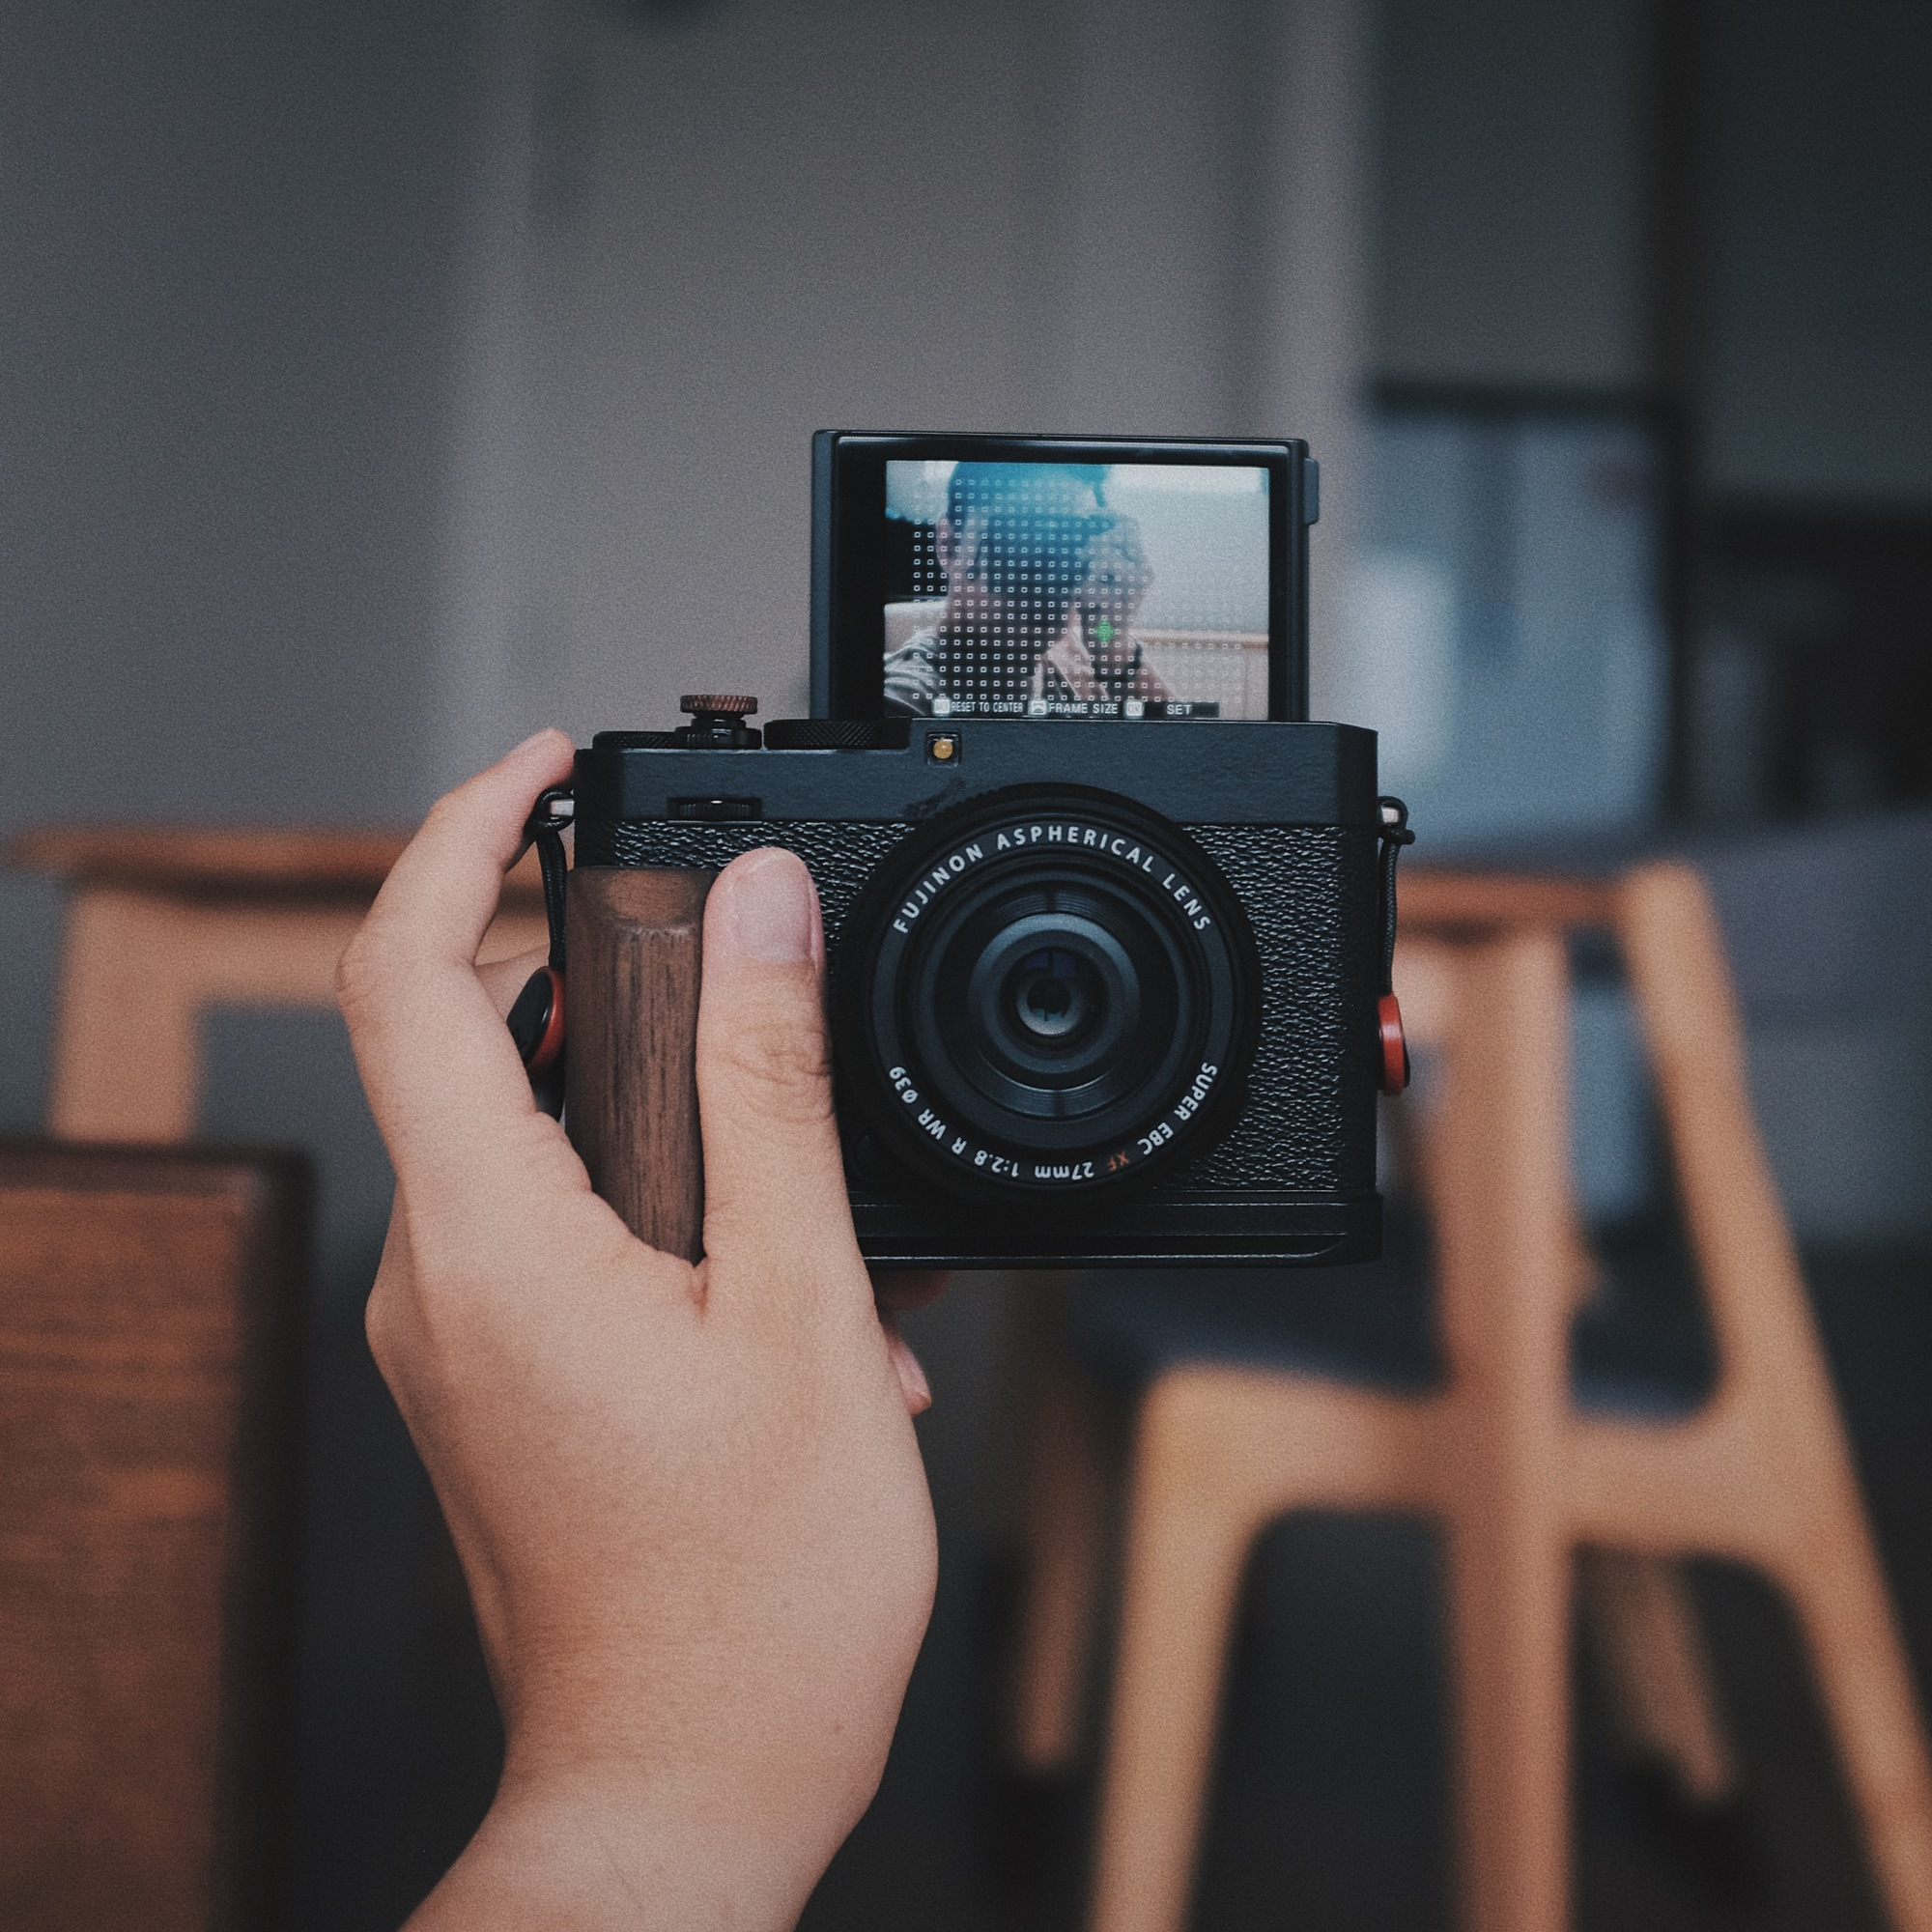
\includegraphics[width=\linewidth]{\envfinaldir/coverpic-prod.jpg}\par
            % \vskip 30pt
            \vfill

            \normalsize\rmfamily\scshape
            \copyright{} The Web Digest Project \hfill\large \envdatestr
        \end{center}
    \end{titlepage}
    % \restoregeometry
}
\newcommand{\simplehref}[1]{%
    \textcolor{blue!80!green}{\href{#1}{#1}}%
}
\renewcommand{\contentsname}{\center\Huge\sffamily\bfseries Contents\par\vskip 20pt}
\newcounter{ipartcounter}
\setcounter{ipartcounter}{0}
\newcommand{\ipart}[1]{
    % \vskip 20pt
    \clearpage
    \stepcounter{ipartcounter}
    \phantomsection
    \addcontentsline{toc}{chapter}{#1}
    % \begin{center}
    %     \Huge
    %     \sffamily\bfseries
    %     #1
    % \end{center}
    % \vskip 20pt plus 7pt
}
\newcounter{ichaptercounter}
\setcounter{ichaptercounter}{0}
\newcommand{\ichapter}[1]{
    % \vskip 20pt
    \clearpage
    \stepcounter{ichaptercounter}
    \phantomsection
    \addcontentsline{toc}{section}{\numberline{\arabic{ichaptercounter}}#1}
    \begin{center}
        \Huge
        \sffamily\bfseries
        #1
    \end{center}
    \vskip 20pt plus 7pt
}
\newcommand{\entrytitlefont}[1]{\subsection*{\raggedright\Large\sffamily\bfseries#1}}
\newcommand{\entryitemGeneric}[2]{
    % argv: title, url
    \parbox{\linewidth}{
        \entrytitlefont{#1}\par\vskip 5pt
        \footnotesize\ttfamily\mdseries
        \simplehref{#2}
    }\vskip 11pt plus 11pt minus 1pt
}
\newcommand{\entryitemGithub}[3]{
    % argv: title, url, desc
    \parbox{\linewidth}{
        \entrytitlefont{#1}\par\vskip 5pt
        \footnotesize\ttfamily\mdseries
        \simplehref{#2}\par\vskip 5pt
        \small\rmfamily\mdseries#3
    }\vskip 11pt plus 11pt minus 1pt
}
\newcommand{\entryitemAp}[3]{
    % argv: title, url, desc
    \parbox{\linewidth}{
        \entrytitlefont{#1}\par\vskip 5pt
        \footnotesize\ttfamily\mdseries
        \simplehref{#2}\par\vskip 5pt
        \small\rmfamily\mdseries#3
    }\vskip 11pt plus 11pt minus 1pt
}
\newcommand{\entryitemHackernews}[3]{
    % argv: title, hnurl, rawurl
    % \parbox{\linewidth}{
    %     \entrytitlefont{#1}\par\vskip 5pt
    %     \footnotesize\ttfamily\mdseries
    %     \simplehref{#3}\par
    %     \textcolor{black!50}{\href{#2}{#2}}
    % }\vskip 11pt plus 11pt minus 1pt
    \begin{minipage}{\linewidth}
            \entrytitlefont{#1}\par\vskip 5pt
            \footnotesize\ttfamily\mdseries
            \simplehref{#3}\par
            \textcolor{black!50}{\href{#2}{#2}}
    \end{minipage}\par\vskip 11pt plus 11pt minus 1pt
}







\begin{document}

\makeheader

\tableofcontents\clearpage




\ipart{Developers}
\ichapter{Hacker News}
\entryitemTwoLinks{Novo Nordisk's Canadian Mistake}{https://news.ycombinator.com/item?id=45637744}{https://www.science.org/content/blog-post/novo-nordisk-s-canadian-mistake}

\entryitemTwoLinks{US Government Uptime Monitor}{https://news.ycombinator.com/item?id=45637049}{https://usa-status.com/}

\entryitemTwoLinks{Airliner hit by possible space debris}{https://news.ycombinator.com/item?id=45636285}{https://avbrief.com/united-max-hit-by-falling-object-at-36000-feet/}

\entryitemTwoLinks{Ask HN: What are people doing to get off of VMware?}{https://news.ycombinator.com/item?id=45635940}{https://news.ycombinator.com/item?id=45635940}

\entryitemTwoLinks{Doing well in your courses: Andrej's advice for success (2013)}{https://news.ycombinator.com/item?id=45635533}{https://cs.stanford.edu/people/karpathy/advice.html}

\entryitemTwoLinks{Thieves steal crown jewels in 4 minutes from Louvre Museum}{https://news.ycombinator.com/item?id=45635528}{https://apnews.com/article/france-louvre-museum-robbery-a3687f330a43e0aaff68c732c4b2585b}

\entryitemTwoLinks{Windows 11 25H2 October Update Bug Renders Recovery Environment Unusable}{https://news.ycombinator.com/item?id=45635287}{https://www.techpowerup.com/342032/windows-11-25h2-october-update-bug-renders-recovery-environment-unusable}

\entryitemTwoLinks{The zipper is getting its first major upgrade in 100 years}{https://news.ycombinator.com/item?id=45634797}{https://www.wired.com/story/the-zipper-is-getting-its-first-major-upgrade-in-100-years/}

\entryitemTwoLinks{With deadline looming 4 of 9 universities reject Trumps pact to remake higher ed}{https://news.ycombinator.com/item?id=45634774}{https://arstechnica.com/culture/2025/10/with-deadline-looming-4-of-9-universities-reject-trumps-compact-to-remake-higher-ed/}

\entryitemTwoLinks{RFCs: Blueprints of the Internet}{https://news.ycombinator.com/item?id=45634678}{https://ackreq.github.io/posts/what-are-rfcs/}

\entryitemTwoLinks{Why an abundance of choice is not the same as freedom}{https://news.ycombinator.com/item?id=45634641}{https://aeon.co/essays/why-an-abundance-of-choice-is-not-the-same-as-freedom}

\entryitemTwoLinks{Xubuntu.org Might Be Compromised}{https://news.ycombinator.com/item?id=45634367}{https://old.reddit.com/r/Ubuntu/comments/1oa4549/xubuntuorg\_might\_be\_compromised/}

\entryitemTwoLinks{Replacement.ai}{https://news.ycombinator.com/item?id=45634095}{https://replacement.ai}

\entryitemTwoLinks{Abandoned land drives dangerous heat in Houston, study finds}{https://news.ycombinator.com/item?id=45634026}{https://stories.tamu.edu/news/2025/10/07/abandoned-land-drives-dangerous-heat-in-houston-texas-am-study-finds/}

\entryitemTwoLinks{Pebble is officially back on iOS and Android}{https://news.ycombinator.com/item?id=45633591}{https://twitter.com/ericmigi/status/1979576965494710564}

\entryitemTwoLinks{OpenAI researcher announced GPT-5 math breakthrough that never happened}{https://news.ycombinator.com/item?id=45633482}{https://the-decoder.com/leading-openai-researcher-announced-a-gpt-5-math-breakthrough-that-never-happened/}

\entryitemTwoLinks{Show HN: Duck-UI – Browser-Based SQL IDE for DuckDB}{https://news.ycombinator.com/item?id=45633453}{https://demo.duckui.com}

\entryitemTwoLinks{What Happened in 2007?}{https://news.ycombinator.com/item?id=45633426}{https://whathappenedin2007.com/}

\entryitemTwoLinks{The case for the return of fine-tuning}{https://news.ycombinator.com/item?id=45633081}{https://welovesota.com/article/the-case-for-the-return-of-fine-tuning}

\entryitemTwoLinks{The Accountability Problem}{https://news.ycombinator.com/item?id=45631678}{https://www.jamesshore.com/v2/blog/2025/the-accountability-problem}\ichapter{Phoronix}
\entryitemGeneric{\hskip 0pt{}Linux 6.18-rc2 Will Make Sure To Wipe Stale Information About AMD System Reboots}{https://www.phoronix.com/news/Linux-6.18-rc2-AMD-Reboot-Info}

\entryitemGeneric{\hskip 0pt{}AYANEO 3 Modular Handheld Console Prepares For Better Linux Support With New Driver}{https://www.phoronix.com/news/AYANEO-3-Linux-Platform-Driver}

\entryitemGeneric{\hskip 0pt{}GCC Front-End Patches Updated For Algol 68 Programming Language}{https://www.phoronix.com/news/Algol-68-GCC-Patches-Updated}

\entryitemGeneric{\hskip 0pt{}Multi-Kernel Architecture Patches Updated For The Linux Kernel}{https://www.phoronix.com/news/Multi-Kernel-Linux-v2}

\entryitemGeneric{\hskip 0pt{}FreeBSD 15.0 Beta 2 Released With Release Building Improvements, New "Blocklist"}{https://www.phoronix.com/news/FreeBSD-15.0-Beta-2}

\entryitemGeneric{\hskip 0pt{}New Code Merged For Linux 6.18 To Address Linus Torvalds' Rust Formatting Critique}{https://www.phoronix.com/news/Linux-6.18-rc2-Rust}

\entryitemGeneric{\hskip 0pt{}Linux Display Driver Patches Posted For The Qualcomm Snapdragon X2 Elite}{https://www.phoronix.com/news/Snapdragon-X2-Display-Support}

\entryitemGeneric{\hskip 0pt{}Tellusim Core SDK Posted On GitHub As C++ SDK For Graphics / Compute}{https://www.phoronix.com/news/Tellusim-Core-SDK-GitHub}

\entryitemGeneric{\hskip 0pt{}Updated Linux Patch Would Disable RDSEED For All AMD Zen 5 CPUs}{https://www.phoronix.com/news/RDSEED-Disable-All-Zen-5}


\ipart{Developers~~~~(zh-Hans)}
\ichapter{Solidot}
\entryitemGeneric{\hskip 0pt{}维基百科称 AI 导致人类访问量下降}{https://www.solidot.org/story?sid=82577}

\entryitemGeneric{\hskip 0pt{}报告称互联网上逾半数内容是 AI 生成的}{https://www.solidot.org/story?sid=82575}

\entryitemGeneric{\hskip 0pt{}椿象腿部器官含有共生真菌}{https://www.solidot.org/story?sid=82574}

\entryitemGeneric{\hskip 0pt{}GZDoom 开源社区因创始人使用 AI 生成代码而分裂}{https://www.solidot.org/story?sid=82573}

\entryitemGeneric{\hskip 0pt{}韩国在四个月试用后放弃了 AI 教科书}{https://www.solidot.org/story?sid=82572}

\entryitemGeneric{\hskip 0pt{}南极洲冰盖出现类似格陵兰岛的加剧融化迹象}{https://www.solidot.org/story?sid=82571}

\entryitemGeneric{\hskip 0pt{}2024 年大气二氧化碳水平创新高}{https://www.solidot.org/story?sid=82570}

\entryitemGeneric{\hskip 0pt{}微软新产品计划在中国之外制造}{https://www.solidot.org/story?sid=82569}

\entryitemGeneric{\hskip 0pt{}Mozilla 测试免费的 Firefox VPN 服务}{https://www.solidot.org/story?sid=82568}

\entryitemGeneric{\hskip 0pt{}Paxos 不小心制造了 300 万亿美元的 PayPal 稳定币}{https://www.solidot.org/story?sid=82567}\ichapter{V2EX}
\entryitemGeneric{\hskip 0pt{}[问与答] 一直收藏的飞书云文档被删除了有什么办法可以联系作者恢复?}{https://www.v2ex.com/t/1166843}

\entryitemGeneric{\hskip 0pt{}[Steam] 今年买的最值的服务}{https://www.v2ex.com/t/1166841}

\entryitemGeneric{\hskip 0pt{}[分享创造] 我用 AI 撸了一个完全无后端免登录的作文学习平台,家里有六年级小孩的可以试一下用来辅导作文。}{https://www.v2ex.com/t/1166840}

\entryitemGeneric{\hskip 0pt{}[分享创造] 最近痴迷音乐类游戏,又做了一个节奏盒子 sprunki,欢迎大家赏脸。。。}{https://www.v2ex.com/t/1166837}

\entryitemGeneric{\hskip 0pt{}[分享发现] 三星 Z Fold 7 vs 谷歌 Pixel 10 Pro Fold 上手体验分享}{https://www.v2ex.com/t/1166836}

\entryitemGeneric{\hskip 0pt{}[摄影] 这种风格的照片是怎么制作出来的?}{https://www.v2ex.com/t/1166835}

\entryitemGeneric{\hskip 0pt{}[分享发现] 真扯淡,自己用 AI 生成小说,竟然看上瘾了。}{https://www.v2ex.com/t/1166834}

\entryitemGeneric{\hskip 0pt{}[宽带症候群] 现在还能用 DDNS 吗?一直访问 IP}{https://www.v2ex.com/t/1166833}

\entryitemGeneric{\hskip 0pt{}[问与答] 完全免费的 claude 工具,真香!}{https://www.v2ex.com/t/1166831}

\entryitemGeneric{\hskip 0pt{}[Windows] 十月安全更新会引发 USB 设备失效问题}{https://www.v2ex.com/t/1166829}

\entryitemGeneric{\hskip 0pt{}[Edge] 鉴于 Edge 疯狂的占用内存, 我只能被迫使用 Safari 了}{https://www.v2ex.com/t/1166828}

\entryitemGeneric{\hskip 0pt{}[Apple] x86 的 mac 还能用多久呢?}{https://www.v2ex.com/t/1166827}

\entryitemGeneric{\hskip 0pt{}[加密货币] 电子支付?}{https://www.v2ex.com/t/1166826}

\entryitemGeneric{\hskip 0pt{}[分享创造] 便宜的 sora2 api}{https://www.v2ex.com/t/1166825}

\entryitemGeneric{\hskip 0pt{}[问与答] 为什么喜欢跑马拉松?}{https://www.v2ex.com/t/1166822}

\entryitemGeneric{\hskip 0pt{}[Apple] 如何让苹果审核人员看到完整功能}{https://www.v2ex.com/t/1166821}

\entryitemGeneric{\hskip 0pt{}[分享创造] MotionFlow:在浏览器中提取 Android 动态照片中的静态图片和视频}{https://www.v2ex.com/t/1166820}

\entryitemGeneric{\hskip 0pt{}[宽带症候群] 全球独一份的中国 eSIM…………}{https://www.v2ex.com/t/1166818}

\entryitemGeneric{\hskip 0pt{}[职场话题] 请教, 正处于迷茫加自我怀疑阶段, 求指导}{https://www.v2ex.com/t/1166817}

\entryitemGeneric{\hskip 0pt{}[酷工作] 招聘: Execution Quant/Desk Quant  APAC Community Lead DevRel Engineer DEX/DeFi 产品经理 RWA 产品经理 Golang 、flutter 、测试、前端}{https://www.v2ex.com/t/1166816}

\entryitemGeneric{\hskip 0pt{}[投资] 人在大陆,除了 ibkr,还有其他买美股的券商可以开户吗}{https://www.v2ex.com/t/1166815}

\entryitemGeneric{\hskip 0pt{}[分享创造] dingtalk-oidc: 一个把钉钉的非标准 OAuth 登陆转换成标准 OIDC 的项目}{https://www.v2ex.com/t/1166814}

\entryitemGeneric{\hskip 0pt{}[问与答] 请问各位大佬,怎么配置合适的机场规则啊?}{https://www.v2ex.com/t/1166813}

\entryitemGeneric{\hskip 0pt{}[问与答] 感觉和别人争论或者吵架很累 很少与别人发生冲突 除非事情特别过分的情况下}{https://www.v2ex.com/t/1166812}

\entryitemGeneric{\hskip 0pt{}[Android] 安卓 15 如何安装旧版 app?}{https://www.v2ex.com/t/1166810}

\entryitemGeneric{\hskip 0pt{}[问与答] Intellij idea windsurf 插件 代码自动提示实效了?}{https://www.v2ex.com/t/1166809}

\entryitemGeneric{\hskip 0pt{}[问与答] V2EX Polish 是不是添加新字体了 网站字体变化了}{https://www.v2ex.com/t/1166808}

\entryitemGeneric{\hskip 0pt{}[职场话题] 华为云 CEO 张平安被连降三等}{https://www.v2ex.com/t/1166807}

\entryitemGeneric{\hskip 0pt{}[Android] 手机疯狂弹录音提醒,还找不到到底是什么应用在使用权限.}{https://www.v2ex.com/t/1166806}

\entryitemGeneric{\hskip 0pt{}[生活] 分享一次飞猪购买火车票的维权经历}{https://www.v2ex.com/t/1166805}

\entryitemGeneric{\hskip 0pt{}[程序员] 预算有限,想入一台 MacBookPro 做开发, M1pro 2025 年还能再战几年?}{https://www.v2ex.com/t/1166804}

\entryitemGeneric{\hskip 0pt{}[问与答] 你在闲鱼上遇到过最无语的事是什么}{https://www.v2ex.com/t/1166803}

\entryitemGeneric{\hskip 0pt{}[分享发现] iPhone 还是可以信赖的,安全,保护隐私。。。}{https://www.v2ex.com/t/1166802}

\entryitemGeneric{\hskip 0pt{}[问与答] 为什么我在 ubuntu22 上用 fio 测试 virtiofs 挂载目录不如 qcow2 虚拟机磁盘的速度呢?}{https://www.v2ex.com/t/1166801}

\entryitemGeneric{\hskip 0pt{}[分享创造] Claude Agent skills 不错,感觉比 mcp 更实用}{https://www.v2ex.com/t/1166799}

\entryitemGeneric{\hskip 0pt{}[程序员] 使用 网站模版+ claude code + glm4.6 撸了一个故事生成网站}{https://www.v2ex.com/t/1166798}

\entryitemGeneric{\hskip 0pt{}[分享创造] 做了个期末成绩计算器,给还在上学的朋友们用}{https://www.v2ex.com/t/1166797}

\entryitemGeneric{\hskip 0pt{}[前端开发] uni-app H5 项目想复用到微信小程序,多端适配与多项目复用怎么设计?}{https://www.v2ex.com/t/1166795}

\entryitemGeneric{\hskip 0pt{}[加密货币] 当前这个阶段哪个冷钱包更好呢}{https://www.v2ex.com/t/1166794}

\entryitemGeneric{\hskip 0pt{}[程序员] 请问有做过小票打印的朋友么,我们最近准备做小票打印,买了个热敏打印机,然后想前端直接调用打印}{https://www.v2ex.com/t/1166792}

\entryitemGeneric{\hskip 0pt{}[MacBook Pro] 我的 mac 笔记本会多出来个 Virtual Display 显示器}{https://www.v2ex.com/t/1166791}

\entryitemGeneric{\hskip 0pt{}[分享发现] 买 apple watch 就是一种病 买完立马继续了}{https://www.v2ex.com/t/1166789}

\entryitemGeneric{\hskip 0pt{}[程序员] CAP 理论里的可用性 A 和分区容错性 P 的区别到底是啥啊?}{https://www.v2ex.com/t/1166788}

\entryitemGeneric{\hskip 0pt{}[分享创造] 鉴于 macOS 看图功能不好用,我自己照着 AI 写了一个}{https://www.v2ex.com/t/1166787}

\entryitemGeneric{\hskip 0pt{}[分享创造] 不想选歌、不想刷推荐,就听``人声''流动}{https://www.v2ex.com/t/1166786}

\entryitemGeneric{\hskip 0pt{}[音乐] 没出息.mp3(非鬼畜版)}{https://www.v2ex.com/t/1166785}

\entryitemGeneric{\hskip 0pt{}[投资] 大饼还是黄鱼?}{https://www.v2ex.com/t/1166784}

\entryitemGeneric{\hskip 0pt{}[Samsung] 三星手机指纹登录支付宝和银河证券会报指纹(生物特征)发生变化然后自动关闭指纹快捷登录}{https://www.v2ex.com/t/1166783}

\entryitemGeneric{\hskip 0pt{}[问与答] macrodroid 宏的问题:在后台时能 log 到动作,但是没能真实开启 app 服务}{https://www.v2ex.com/t/1166781}

\entryitemGeneric{\hskip 0pt{}[游戏开发] [游戏] 鸡排主理人,来体验主理人的忙碌吧}{https://www.v2ex.com/t/1166779}


\ipart{Generic News}







\clearpage
\leavevmode\vfill
\footnotesize

Copyright \copyright{} 2023-2025 Neruthes and other contributors.

This document is published with CC BY-NC-ND 4.0 license.

The entries listed in this newsletter may be copyrighted by their respective creators.

This newsletter is generated by the Web Digest project.

The newsletters are also delivered via Telegram channel \CJKunderline{\href{https://t.me/webdigestchannel}{https://t.me/webdigestchannel}}.\\
RSS feed is available at \CJKunderline{\href{https://webdigest.pages.dev/rss.xml}{https://webdigest.pages.dev/rss.xml}}.

This newsletter is available in PDF at
\CJKunderline{\href{https://webdigest.pages.dev/}{https://webdigest.pages.dev/}}.

The source code being used to generate this newsletter is available at\\
\CJKunderline{\href{https://github.com/neruthes/webdigest}{https://github.com/neruthes/webdigest}}.

This newsletter is also available in
\CJKunderline{\href{http://webdigest.pages.dev/readhtml/\envyear/WebDigest-20251020.html}{HTML}} and
\CJKunderline{\href{https://github.com/neruthes/webdigest/blob/master/markdown/\envyear/WebDigest-20251020.md}{Markdown}}.


\coverpic{https://unsplash.com/photos/couple-embracing-in-front-of-a-historic-cathedral-4ddJMEc4wAs}{Karsten Winegeart}


\end{document}
